\section{Architectures à mémoire partagée}\label{sec:context:numa}


Les architectures à mémoire partagée ont subi des changements majeurs liés à l'évolution des processeurs.
L'augmentation du nombre de cœurs par processeur a introduit des problèmes d'accès à la mémoire centrale : dans une architecture composée d'une unique mémoire, plusieurs cœurs cherchant à accéder à la mémoire vont rentrer en concurrence et introduire de la contention et donc des délais dans l'accès à la mémoire, ce qui pénalise fortement les performances.

Pour pallier ce problème, les constructeurs ont divisé la mémoire centrale en plusieurs parties physiquement distinctes, appelées \emph{nœuds}.
Le nœud NUMA est le composant de base pour une architecture NUMA.
Chaque nœud est constitué d'une partie de la mémoire centrale, d'un contrôleur local d'accès à ce bloc mémoire, ainsi que d'un certain nombre de processeurs multicœurs, eux-mêmes composés de plusieurs cœurs de calcul.
L'ensemble des nœuds de la machine sont ensuite reliés entre eux par un réseau d'interconnexion.
La topologie de l'interconnexion ne permet généralement pas d'avoir des nœuds équidistants, ce qui introduit une hiérarchie mémoire.

Malgré le fait que les différentes parties de l'architecture soient physiquement séparées, le système d'exploitation voit l'ensemble comme une unique machine.

Nous décrivons dans un premier temps, dans la section~\ref{sec:context:numa:multicore}, les caractéristiques techniques communes des processeurs multicœur consituant les nœuds NUMA, puis celles des systèmes d'interconnexion des nœuds dans la section~\ref{sec:context:numa:interconnect}.
Elles ont une influence directe sur le comportement du nœud au sein de la machine.

\subsection{À l'intérieur d'un processeur multicœur}\label{sec:context:numa:multicore}

Les sections suivantes se concentrent sur certains composants clés des performances d'un processeur multicœur.
Les fréquences des cœurs des processeurs sont beaucoup plus élevées que celles des bus d'accès à la mémoire centrale.
Cela implique a priori que le temps d'exécution du programme va être limité par le temps d'accès à la mémoire (phénomène introduit sous le nom de \emph{Memory Wall}~\cite{Wulf1995}).
L'architecture des caches et leurs caractéristiques sont cruciales pour limiter l'impact de ce phénomène, nous les abordons en détail dans la section~\ref{sec:context:numa:cache}.
La section~\ref{sec:context:numa:node} décrit le parallélisme que les processeurs peuvent exposer pour augmenter les performances, via des instructions ou composants matériels spécifiques.



\subsubsection{Des caches pour accélérer l'accès aux données}\label{sec:context:numa:cache}

Le cache est une mémoire pour laquelle le temps d'accès est bien meilleur que pour la mémoire centrale, mais dont la capacité est beaucoup plus restreinte. Il peut être spécifique à un cœur du processeur, ou partagé par plusieurs d'entre eux.

\paragraph{Fonctionnement}

Au niveau des accès, le fonctionnement d'un cache est légèrement différent de celui de la mémoire centrale : plutôt que de pouvoir adresser uniquement un octet, c'est généralement une partie fixe de la mémoire contenant cet octet qui est chargée.
On appelle cette quantité une \emph{ligne de cache}, et un exemple de taille standard pour une ligne de cache est 64 octets (8 nombres réels double précision).

Lorsqu'une instruction demande le chargement d'une valeur située en mémoire, le contrôleur du cache reçoit la requête du processeur, détermine la ligne de cache correspondante à partir de l'adresse demandée, et effectue l'une des deux opérations suivantes :
\begin{description}
  \item [Cache hit :] si la ligne correspondante est déjà présente dans le cache, la donnée est directement retournée au cœur.
  \item [Cache miss :] si la ligne n'est pas présente, le contrôleur de cache va charger la valeur depuis la mémoire centrale ou un autre niveau de cache, et retourner la valeur au cœur.
\end{description}

%(je vire ça vu qu'on ne parle de niveaux de cache que plus tard) Si le cœur a accès à plusieurs niveaux de cache, la requête est transférée au niveau supérieur, et seul le dernier niveau effectue la requête à la mémoire centrale.
Une fois qu'une ligne est chargée dans le cache, elle n'y reste pas de manière permanente, plusieurs raisons décrites ci-après peuvent entraîner son \emph{éviction} du cache~:

\begin{itemize}
  \item Le maintien de la cohérence : lorsqu'un cœur modifie une ligne de cache dans son propre cache, cette même ligne est \emph{invalidée} dans les caches des autres processeurs qui disposent d'une version de celle-ci.
Si un processeur essaie de faire un accès sur une ligne invalidée, elle sera rechargée depuis la mémoire centrale ou un autre cache en possédant une copie valide, générant un \emph{cache miss}.
  \item Le dépassement de la capacité du cache : il est assez commun que l'ensemble des données manipulées par le programme ne tienne pas dans le cache.
Lorsqu'une requête est effectuée sur une ligne, qu'elle n'est pas présente dans le cache, et que le cache est plein, le contrôleur choisira une ligne à évincer du cache pour faire de la place à la nouvelle ligne.
Le choix de la ligne à évincer est un sujet très étudié, et le prochain paragraphe revient sur les politiques d'éviction communément utilisées.
  \item Le conflit d'adresse : dans la quasi totalité des modèles de caches, certaines lignes correspondant à des adresses mémoires doivent être stockées dans le même emplacement du cache.
    Si elles sont requises alternativement pendant l'exécution du programme, elles se sortiront mutuellement du cache.
    Ce problème dépend directement de l'\emph{associativité} du cache, qui est traitée dans le paragraphe suivant.
\end{itemize}



\paragraph{Associativité}

Le cache ne peut être suffisamment grand pour contenir toute la mémoire~: le temps d'accès est lié à sa taille, et sa taille est généralement négligeable face à la quantité totale de mémoire disponible.
Néanmoins chaque partie de la mémoire doit pouvoir être stockée dans une partie du cache, il faut donc pouvoir déterminer l'association entre l'adresse d'une ligne dans la mémoire centrale et son emplacement dans le cache.
L'associativité du cache varie entre une association directe (\emph{direct-mapped cache}), où chaque ligne de la mémoire est associée à exactement un emplacement dans le cache~; et une association complète (\emph{fully associative cache}), où chaque ligne de la mémoire peut être associée à n'importe quel emplacement dans le cache.

Hill et al.~\cite{Hill1989} illustrent l'impact de l'associativité (dans la table III de l'article) sur la proportion de \emph{cache miss} et catégorise son origine (conflit d'adresse, défaut de capacité du cache, chargement normal de la donnée).
Cela permet de dégager deux observations : d'une part qu'augmenter l'associativité permet de diminuer les \emph{cache miss}.
D'autre part que les défauts de cache ayant une forte associativité sont quasi exclusivement dus à la capacité du cache, alors que pour les caches à association directe les conflits d'adresse sont une part non négligeable des \emph{cache miss}.

\paragraph{Niveaux de caches}

Il y a en général 3 niveaux de caches dans ces architectures, labellisés L1, L2, et L3.
La figure~\ref{fig:context:schema-caches} décrit la hiérarchie typique d'un processeur multicœurs que l'on peut trouver sur un nœud NUMA.

Le L1 est privé au cœur, il est découpé en deux parties~: une spécifique aux données, et l'autre aux instructions. C'est le niveau de cache le plus proche du CPU mais aussi le plus petit~: seulement 32 Ko dans cet exemple.
Le cache L2 est lui aussi privé au cœur, mais propose une plus grande capacité (ici 256 Ko) au prix d'une latence plus importante.
Enfin le cache L3, ou cache de dernier niveau - \emph{Last Level Cache (LLC)}, est partagé par tous les cœurs du processeur. La latence pour y accéder est plus importante que pour accéder au L2, mais sa capacité est bien supérieure, atteignant en général plusieurs Mo, 20 dans cet exemple.

\begin{figure}[ht]
  \centering
  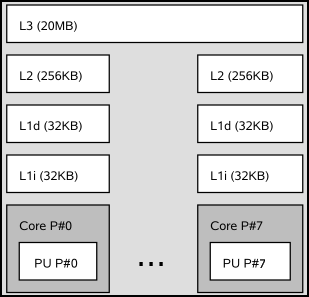
\includegraphics{processor_small}
  \caption{Schéma d'un processeur multicœurs}\label{fig:context:schema-caches}
\end{figure}

En général les développeurs d'applications pour le HPC accordent beaucoup d'attention à l'optimisation de leur application, pour que les parties de code séquentiel critiques utilisent des données qui puissent être contenues dans le L1/L2.
De même, beaucoup d'optimisations au sein des compilateurs visent également cet objectif.

Lorsqu'il s'agit de cibler des architectures NUMA, on va tout particulièrement s'intéresser au L3 qui représente la mémoire la plus rapide accessible par tous les cœurs d'un même nœud, et donc faire attention à ce que les données qui sont partagées par plusieurs cœurs puissent être contenues dans ce cache.

\begin{table}[ht]
\def\arraystretch{1.5}
\centering
\begin{tabular}{|c||c|c|c|c|}\hline
  Cache & \multicolumn{2}{c|}{Intel Sandy Bridge (2012, idchire)} & \multicolumn{2}{c|}{Intel Broadwell (2016, brunch)}  \\ \cline{2-5}
 & Latence & Bande passante & Latence & Bande passante \\ \hline
 L1 & 1.6 ns & 16 Go/s & 1.8 ns & 32 Go/s \\ \hline
 L2 & 5.0 ns & 14 Go/s & 5.4 ns & 17 Go/s \\ \hline
 L3 & ~20 ns & 8 Go/s & ~24 ns & 9 Go/s \\ \hline
 RAM & ~90 ns & 4 Go/s & ~140 ns & 7 Go/s \\ \hline
 RAM distante & ~500 ns & 1.1 Go/s & ~230ns & 4.2 Go/s \\ \hline
\end{tabular}
\caption{Tableau synthétique des latences et bandes passantes en fonction du niveau de cache et du processeur}\label{tab:synthese-processeurs}
\end{table}

Afin de donner un ordre d'idée des latences et bandes passantes sur les différents processeurs, le tableau~\ref{tab:synthese-processeurs} récapitule les chiffres en fonction de la génération du processeur.
Nous avons fait ces mesures à l'aide de l'outil LMbench~\cite{McVoy1996}. Pour la latence, les débits considérés sont ceux du benchmark |lat_mem_rd| avec un accès aléatoire à la mémoire.
Pour la bande passante les temps considérés sont ceux du benchmark |bw_mem|, en utilisant un équivalent de |memcpy|.
La majorité des processeurs dotés d'un cache dispose également d'un composant matériel - le \emph{prefetcher} - dont le but est de charger en avance des données dans le cache en fonction des accès déjà effectués aux données.
Pour la latence, tout effet potentiel de ce composant est annulé par l'utilisation de \emph{pointer chasing} (l'adresse de la case suivante à charger est située dans la case courante), ce qui n'est pas le cas pour la bande passante.

Comme nous pouvons le voir sur ces chiffres, le coût d'accès à la mémoire principale est bien plus grand que l'accès des différents caches, et l'accès à la mémoire distante est tout simplement prohibitif.
Il faut également noter une évolution intéressante au niveau des latences~: bien que Broadwell soit une architecture plus récente que Sandy Bridge, les latences aux différents niveaux de caches sont plus élevées, sauf pour l'accès à la mémoire distante où elle a été diminuée de moitié.
Les différentes caractéristiques de ces processeurs et des machines sur lesquelles ils sont intégrés seront étudiées en détails dans la section~\ref{sec:contribs:machines}.


\paragraph{Politiques d'éviction}

Le choix de la ligne de cache à remplacer lorsque le cache est plein a un impact direct sur les performances, et les politiques de remplacement ont été très étudiées par les différents acteurs de la communauté académique et industrielle.
Le choix de la politique dépend de multiple facteurs, tels que la taille du cache, son associativité, ou l'espace matériel disponible pour la réaliser.
Al-Zoubi et al.~\cite{Al-Zoubi2004} proposent une évaluation complète et détaillée de l'impact des politiques d'éviction en fonction de l'associativité du cache.
Dans cette évaluation, des variations de la politique Pseudo-LRU semblent être les plus avantageuses pour les associativités étudiées.
Le coût d'implémentation de la politique \emph{Least Recently Used (LRU)} devient trop important lorsque l'associativité dépasse un certain seuil~\cite{Kedzierski2010}~; Pseudo-LRU offre une alternative où la ligne choisie pour être évincée est une parmi celles utilisées il y a le plus longtemps.

Dans les processeurs Intel, des variantes de la politique Pseudo-LRU semble être les plus utilisées pour les caches de faibles associativités, et donc typiquement les caches de niveaux L1 et L2~\cite{Abel2014,IntelXeonPhi2014}.
Dans le cas spécifique du cache de dernier niveau (LLC), certains fabricants comme Intel utilisent des politiques adaptatives présentées comme supérieures à Pseudo-LRU, prenant en compte la fréquence à laquelle sont utilisées certaines lignes de caches.
\emph{Dynamic Re-Referency Interval Prediction} en est un exemple, qui a été présenté parmi d'autres par Jaleel et al.~\cite{Jaleel2010}.
D'autres constructeurs tels que ARM font le choix de la simplicité d'implémentation, comme par exemple dans les processeurs ARM Cortex-R~\cite{ARM-Cortex-R}, où le choix de la ligne à évincer est tout simplement aléatoire.

\subsubsection{Du parallélisme au sein du processeur pour augmenter la puissance de calcul}\label{sec:context:numa:node}

En plus des caches qui nous intéresseront tout particulièrement dans la suite de ce manuscrit, les processeurs ont également d'autres composants matériels dont il est important d'avoir conscience, mais qui ont une place plus limitée dans le contexte de cette thèse : il s'agit des instructions vectorielles et de l'hyperthreading, décrit ci-après.

\paragraph{Instructions vectorielles}\label{sec:context:numa:simd}

Le concept de vectorisation est l'action d'appliquer une même instruction sur plusieurs données (ou un \emph{vecteur} de données) nécessitant la même opération.
Ce type d'instructions est appelé SIMD, pour \emph{Single Instruction Multiple Data}~\cite{Flynn1966}.
La vectorisation permet au processeur d'optimiser la décomposition de l'instruction en micro opérations et donc l'utilisation du pipeline des différentes Unité Arithmétique et Logique (UAL)~\cite{Muller1989}.

Des extensions au jeu d'instructions x86 ont été créées afin de pouvoir opérer sur des éléments plus larges que 64 bits, et la plupart des architectures des processeurs récents utilisent des registres plus larges que le type le plus large en C (|long long|, 64 bits).
La première d'entre elles, SSE (\emph{Streaming SIMD Extensions}), a été introduite par Intel dès 1999 et a évolué régulièrement, agrandissant progressivement la taille des registres jusqu'à l'extension AVX-512, permettant d'effectuer des instructions sur des registres de 512 bits.

La plupart des processeurs actuels (depuis les Sandy Bridge d'Intel, et les Bulldozer d'AMD, en 2011) supportent au moins l'extension AVX avec des registres de 128 bits.

\paragraph{Hyperthreading}

Chaque cœur possède un certain nombre d'UALs qui lui sont privées. Lorsqu'il est en attente d'une donnée de la mémoire centrale, ces UALs ne sont pas utilisées, et des cycles CPU sont donc "perdus" à ne rien faire.

Afin de maximiser l'utilisation de ces ressources, certains processeurs Intel sont équipés de la technologie \emph{hyperthreading}.
Le concept est assez simple : avoir deux cœurs logiques (\emph{hyperthreads}) associés à un seul cœur physique.
De cette manière lorsqu'un thread est en attente sur une donnée (par exemple lors d'un chargement d'une donnée depuis la mémoire), le second peut éventuellement profiter des UALs disponibles.

Pour des tâches peu gourmandes en ressources ou utilisant beaucoup de données, cela peut effectivement se traduire par un gain de performance, mais dans le cadre du calcul haute performance il faut regarder le type d'applications utilisé pour savoir si on peut espérer un gain ou non.
En particulier les caches L1 et L2 sont partagés par les deux hyperthreads, donc si le code séquentiel généré est optimisé pour les tailles de caches correspondant, exécuter le même type de code séquentiel sur deux hyperthreads peut entrainer du \emph{cache trashing}.
Au meilleur des cas l'hyperthreading améliorera les performances~: Jeffers et al.~\cite{Jeffers2016} rapportent par exemple entre 2.3 et 3.3 de speed-up pour 4 hyperthreads par cœur sur les derniers processeurs d'Intel, les Xeon Phi.
Si l'application est très intensive en calcul et utilise au maximum les UALs, l'hyperthreading n'apportera pas grand chose, voire rien.

L'hyperthreading est généralement une option que l'on peut désactiver dans le BIOS de la machine, ou éviter en plaçant correctement les threads de son application.


\subsection{Passage à l'échelle supérieure : interconnexion des processeurs}\label{sec:context:numa:interconnect}

L'une des parties majeures d'une machine NUMA est le système d'interconnexion entre les différents nœuds.
C'est cette partie qui va déterminer à quel point cela va être couteux d'accéder à la mémoire située sur un nœud distant, et donc à quel point l'aspect NUMA de la machine va impacter les performances d'une application.
Dans la majorité des cas, ce système d'interconnexion est \emph{cache-coherent}, c'est à dire que la cohérence de cache est assurée entre les différents nœuds par le matériel, et n'est pas la responsabilité du programmeur ou du support exécutif.
L'impact sur les performances peut être lié à la fois au protocole de cohérence de cache utilisé, ainsi qu'à la topologie de l'interconnexion des nœuds.


\subsubsection{Protocoles de cohérence de cache}

Le nombre de caches utilisés dans une machine NUMA peut être important, et la même ligne de la mémoire peut être présente dans plusieurs caches en même temps.
Il est important que l'état des différentes copies soit cohérent : par exemple si une ligne a été écrite et modifiée, les copies de cette ligne dans les autres caches doivent être mises à jour.

La plupart des protocoles se basent sur un ensemble d'états possibles pour une ligne de cache :

\begin{description}
  \item [Modified (M) :] la ligne a été modifiée dans le cache. Les données dans cette ligne ne sont donc pas cohérentes avec la mémoire principale. Quand la ligne est évincée, elle doit être écrite dans la mémoire principale.
  \item [Shared (S) :] la ligne est <<propre>> (non modifiée), elle existe dans d'autres caches mais est en lecture seule dans le cache courant. Cette ligne peut être évincée sans autre action.
  \item [Invalid (I) :] la ligne est soit absente du cache courant ou a été invalidée par un autre cache. Elle doit être récupérée depuis la mémoire principale (ou un autre cache qui en possède une copie valide).
\end{description}

Cet ensemble d'états de base forme le protocole \emph{MSI}, qui a ensuite été étendu avec plusieurs autres états :

\begin{description}
  \item [Exclusive (E) :] la ligne est présente uniquement dans le cache courant et elle est <<propre>>.
  \item [Owned (O) :] la ligne est présente dans plusieurs caches dans un état valide, mais seul le cache courant peut y effectuer des modifications.
    Cet état permet de partager des lignes qui ont été modifiées sans passer par une ré-écriture dans la mémoire centrale : le cache qui possède la ligne est responsable de fournir une version à jour, et d'écrire la ligne dans la mémoire centrale lorsque que la ligne est évincée.
  \item [Forward (F) :] cet état est similaire à l'état \emph{Shared}, mais indique au cache courant qu'il est responsable de satisfaire une requête en lecture sur la ligne.
\end{description}

Intel Quick Path Interconnect~\cite{Ziakas2010} (QPI) est le système d'interconnexion utilisé dans les machines d'expérimentation que nous avons utilisées, et qui sont décrites dans la section~\ref{sec:contribs:machines}.
Il implémente le protocole MESIF. Du à l'introduction de l'état \emph{F}, ce protocole est avantageux lorsque la latence de cache à cache est bien plus faible que la latence d'accès à la mémoire principale.
AMD HyperTransport~\cite{Keltcher2003} est le système d'interconnexion utilisé dans les machines à base de processeurs AMD, et implémente le protocole MOESI.

Pour implémenter ces protocoles, il existe deux types de mécanismes :

\begin{itemize}
  \item À base de Snooping : chaque cache observe le trafic sur le bus mémoire pour des requêtes qui concerneraient les lignes de caches dont il possède une copie. Un composant dédié peut effectuer un premier filtre pour restreindre le trafic lié au mécanisme de snooping. Néanmoins ce type de mécanismes ne passe pas bien à l'échelle, et aurait du mal à obtenir de bonnes performances dans les architectures NUMA, où le nombre de caches est important.

  \item À base de répertoires : la donnée est placée dans un répertoire qui maintient la cohérence entre les caches. Les caches ne peuvent pas accéder directement à la mémoire principale mais doivent passer par le répertoire.
\end{itemize}

Le QPI utilise un mix des deux mécanismes : il utilise des \emph{home agents} - comparables à des répertoires - qui sont les principales autorités pour fournir une version du cache depuis la mémoire principale.
Il utilise ensuite du \emph{snooping} pour satisfaire les requêtes des différents \emph{caching agents} (les entités qui possèdent un cache, telles que les processeurs).

Le QPI peut fonctionner avec deux modes de \emph{snooping} :
\begin{description}
  \item [Source snooping :] le \emph{caching agent} envoie la requête à tout le système. Les autres \emph{caching agents} peuvent répondre à la requête s'ils possèdent une version de la ligne de cache dans un état compatible. Le \emph{home agent} responsable de la ligne mémoire doit fournir une copie propre de la ligne de cache si besoin, et résoudre les conflits s'ils apparaissent.
  \item [Home snooping :] le \emph{caching agent} envoie la requête au \emph{home agent}, qui envoie ensuite une requête aux \emph{caching agents} qui possèdent une copie de la ligne et peut commencer à charger la ligne depuis la mémoire. L'un des \emph{caching agents} possédant la ligne et/ou le \emph{home agent} peut ensuite envoyer la réponse.
\end{description}

Le mode \emph{source snooping} a une latence plus faible que le mode \emph{home snooping}, mais passe moins bien à l'échelle.
C'est donc ce dernier qui est le plus adapté à un environnement NUMA, puisqu'il limite le nombre de requêtes envoyés sur le bus mémoire, et économise donc de la bande passante.

% NOTE : j'ai pas pu obtenir de réponse sur le mode d'idchire.

\subsubsection{Topologies}

La topologie du système d'interconnexion peut être très différente d'une machine à une autre, et de multiples exemples existent dans les machines commercialisées.
L'objectif de l'interconnexion est de proposer à un maximum de nœuds d'être en lien les uns avec les autres, tout en minimisant la <<distance>> entre eux.
Il existe des topologies plates, où chaque nœud est directement connecté aux autres, comme c'est le cas pour la machine \emph{brunch} décrite en détails dans la section~\ref{sec:contribs:machines:brunch}, mais également des topologies plus compliquées, où par exemple des couples de nœuds sont groupés entre eux et peuvent passer par un ou deux niveaux d'interconnexion, comme c'est le cas pour la machine \emph{idchire}, décrite en détail dans la section~\ref{sec:contribs:machines:idchire}.

Pour illustrer la complexité et l'impact que peut avoir la topologie, prenons l'exemple de la machine \emph{idchire} dont une partie de la topologie est illustrée dans la figure~\ref{fig:context:group-idchire}.
La figure montre 2 nœuds NUMA sur un même groupe, la machine possède en tout 12 groupes (et donc 24 nœuds) interconnectés.

\begin{figure}[ht]
  \centering
  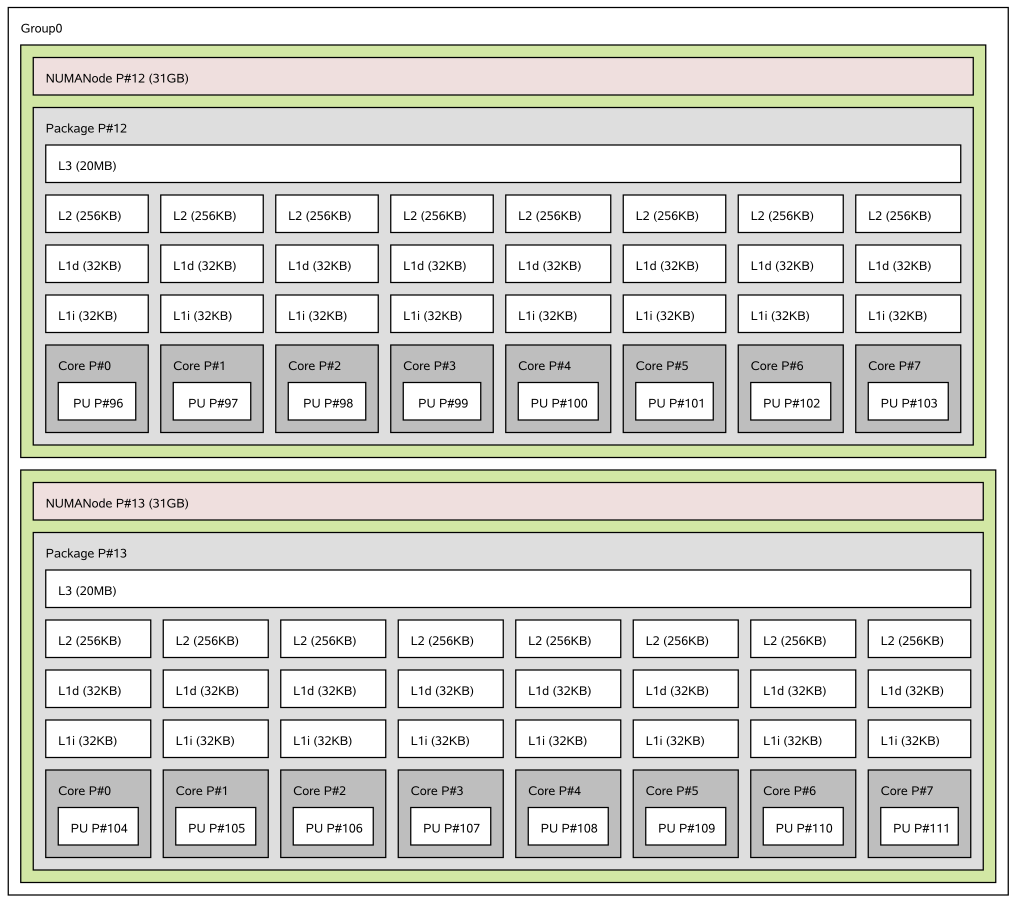
\includegraphics[width=\textwidth]{group}
  \caption{Schéma d'un groupe de deux nœuds sur \emph{idchire}}\label{fig:context:group-idchire}
\end{figure}


Physiquement accéder aux nœuds 1, 2, et 10 depuis le nœud 0 n'est pas équivalent, et les données passent par des liaisons physiques différentes.
Le rapport entre le coût d'accès à un nœud distant et le coût d'accès au nœud local s'appelle le \emph{facteur NUMA}.
Le nombre de rebonds - \emph{hops} - à effectuer avant d'accéder à la mémoire demandée impacte directement la latence et la bande passante.

Une carte complète - \emph{heatmap} - des distances est montrée dans le chapitre~\ref{chap:contrib:characterization}, Figure~\ref{fig:contribs:machines:idchire:heatmap}.
Le tableau~\ref{tab:topologie-hops} donne un comparatif avec des chiffres indicatifs. Nous pouvons constater que sur \emph{idchire} les bandes passantes distantes sont relativement similaires comparativement à la bande locale, qui est presque trois fois plus importante.
Sur une architecture plus récente, \emph{brunch}, la différence de bande passante est bien moindre mais toujours présente.
Ces chiffres motivent fortement l'intérêt à porter à la localité des données.


\begin{table}[ht]
\def\arraystretch{1.5}
\centering
\begin{tabular}{|c||c|c|}\hline
  Destination & idchire & brunch  \\ \hline
 Local & 3.1 Go/s & 3.6 Go/s \\ \hline
 Même groupe & 1.27 Go/s & NA \\ \hline
 1 hop & 1.12 Go/s & 3.2 Go/s \\ \hline
 2 hops & 1.0 Go/s & NA \\ \hline
\end{tabular}
\caption{Bande passante (\emph{memcpy} de 200 Mo) en fonction du nœud destinataire de la copie}\label{tab:topologie-hops}
\end{table}

\bigskip

Cette partie s'est concentrée sur les connaissances de base nécessaires pour comprendre l'interaction entre les différents composants des architectures NUMA.
Le développeur d'application ne va généralement pas influer directement sur ces composants, en revanche il est capital d'avoir conscience des caractéristiques de chacun d'entre eux pour pouvoir expliquer facilement tel ou tel comportement de l'application.

Le premier composant logiciel qui va s'intéresser à la gestion directe du matériel est le système d'exploitation.
La section suivante revient sur les points relatifs à la gestion des architectures NUMA dans le système d'exploitation.
